\section{UPPAAL CORA}\label{sec:upp_cora}
UPPAAL \acrfull{cora} is a branch of UPPAAL, that uses linearly priced timed automata to find optimal paths satisfying certain goals, based on lowest accumulated cost\cite{cs_cora}. Cost is a variable that can be only be interacted with through locations, where it is possible to define the incremental rate with which it will grow, with the passing of time. It allows \gls{cora} to prune traces, if two traces reach the same location where all variables for each of the traces are identical expect for the cost variable, the trace with the lowest cost will be kept to preserve memory. Due to the underlying structure of \gls{cora} it is only possible to do simple reachability checks, and does not allow for liveness checks such as deadlocks. Only best first search is support when using cost and cost is not allow to be used in an expression\ofx{tydeliggør dette}. Lastly \gls{cora} cannot guarantee termination unless the modelled system is acyclic and clocks are bound by invariants.

\Gls{cora} have been used in a range of problems regarding scheduling problems, the most related case for our problem is GomX-3 case, where they used \gls{cora} to generate a battery aware schedule for CubeSat satellite. Their solution takes a set of parameters to generate fractions of the entire schedules and, when all parts of the schedule is generated, they are assembled by appending them in a chronological order. Lastly, the acummulated schedule is tested with an external \gls{kibam} battery model.

\Gls{cora} introduced the concept of cost, which as mentioned is accumulated over time. An example of how such a model may look can be seed in \cref{fig:cora_eks}.

%\begin{figure}[h]
%\begin{centering}
%	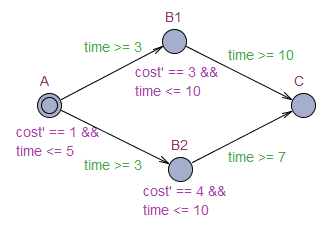
\includegraphics[width=7cm]{graphics/cora_eks.png}
%	\label{fig:cora_eks}
%	\caption{Simple model made in \gls{cora}, which displays an increase in cost over time}
%\end{centering}
%\end{figure}

\begin{figure}
	\centering
	\begin{tikzpicture}
	%Locations
	\node [init] (l0) [label={
		[align=left]above:
		\textcolor{name}{A}
	}, label={
		[align=left]left:
		\textcolor{invariant}{cost '== 1}\\
		\textcolor{invariant}{\&\& time <= 5}
	}] {};
	\node [location] (l1) [right of=l0, xshift=20mm, yshift=20mm, label={
		[align=left]above:
		\textcolor{name}{B1}
	}, label={
		[align=left]below:
		\textcolor{invariant}{cost '== 1}\\
		\textcolor{invariant}{\&\& time <= 5}
	}] {};
	\node [location] (l2) [right of=l0, xshift=20mm, yshift=-20mm, label={
		[align=left]above:
		\textcolor{name}{B2}
	}, label={
		[align=left]below:
		\textcolor{invariant}{cost '== 1}\\
		\textcolor{invariant}{\&\& time <= 5}
	}] {};
	\node [location] (l3) [right of=l2, xshift=20mm, yshift=20mm, label={
		[align=left]above:
		\textcolor{name}{C}
	}, label={
		[align=left]right:
		\textcolor{invariant}{cost '== 1}\\
		\textcolor{invariant}{\&\& time <= 5}
	}] {};
	%Edges
	\path[->,black] (l0) edge node [midway, left][align=left]{
			\textcolor{guard}{time >= 3}} (l1);
	\path[->,black] (l0) edge node [midway, left][align=left]{
			\textcolor{guard}{time >= 3}} (l2);
	\path[->,black] (l1) edge node [midway, right][align=left]{
			\textcolor{guard}{time >= 10}} (l3);
	\path[->,black] (l2) edge node [midway, right][align=left]{
			\textcolor{guard}{time >= 7}} (l3);
	\end{tikzpicture}
	\caption{Simple model made in \gls{cora}, which displays an increase in cost over time}
	\label{fig:cora_eks}
\end{figure}

In \cref{fig:cora_eks} we see a \gls{cora} model with four locations and four edges connecting them. On three of the location there is an invariant bound to the clock "\uppVar{time}" and an associated cost rate. While in the initial location "\uppLoc{A}" the cost rate is one meaning that for every unit of time spend in this \uppLoc{A} the cost will increase by one, it will stay in \uppLoc{A} for three to five units of time before moving on to the next location.\\
After this is where the model gets interesting, there are at this point two possible transitions, it may move to either "\uppLoc{B1}" or "\uppLoc{B2}". In \uppLoc{B1} the cost will increase with a rate of 3 per unit of time and will stay there until time reaches ten. Alternatively it may transition to \uppLoc{B2} where the cost rate is four and will stay there until time is between seven and ten. After visiting one of these locations it will reach the final state "\uppLoc{C}". \\
In UPPAAL we can then run the query seen in \cref{eq:cora_get_c}, a simple query asking if location \uppLoc{C} is reachable, however in \gls{cora} the settings for diagnostic trace allows us to get the best trace, meaning the one with the smallest cost.
\begin{align}
E<> Template.C
\label{eq:cora_get_c}
\end{align}
This is beneficial as the optimal route may not always be the obvious one. We see in \cref{fig:cora_eks} that \uppLoc{B1} only have a cost of three per tic whereas \uppLoc{B2} have a cost of four per tic, however it is required to stay in \uppLoc{B1} for a longer period of time, actually causing the bottom route to become cheaper.
The model in \cref{fig:cora_eks} is of course a simple one,

%This can be advantageous for modelling systems such as satellites where energy is an important and limited resource which can be represented by the cost. After running a query it is possible to extract a trace, which can be used to represent the generated schedule.

%http://people.cs.aau.dk/~adavid/cora/download.html#download


%optimal sceduling and planning.
%state-space exploration -> promising and cheap visited first -> prune parts of search tree not improving solution.
%symbolic data structure -> symbolic state-space representation with cost information -> optimal or near-optimal solutions

%S2,3: problem of cost-optimal reachability -> symbolic branch-and-bound solving this problem.
% clocks are non-negative real values, can be reset and grow at a fixed rate.

%S5: PTA-related optimization problems -> future support

